\documentclass[krantz1,ChapterTOCs]{krantz}
\usepackage{fixltx2e,fix-cm}
\usepackage{amssymb}
\usepackage{amsmath}
\usepackage{subfigure}
\usepackage{makeidx}
\usepackage{multicol}
\usepackage{qrcode}
\usepackage[makeroom]{cancel}
\usepackage{graphicx,pgfplots}
\usepackage{catchfile}
\usepackage[noend]{algpseudocode}
\usepackage{mathtools}
 
\newcommand{\df}[1]{\,\mathrm{d}#1}
\newcommand{\parcial}[3]{\dfrac{\partial^{#1}#2}{\partial #3^{#1}}}
\newcommand{\getenv}[2][]{%
    \CatchFileEdef{\temp}{"|kpsewhich --var-value #2"}{\endlinechar=-1}%
    \if\relax\detokenize{#1}\relax\temp\else\let#1\temp\fi}
\getenv[\BIBREF]{RM_REFERENCES}

\newcommand{\eq}[1]{Equação (\ref{#1})}
\newcommand{\fig}[1]{Figura (\ref{#1})}
\newcommand{\algo}[1]{Algoritmo (\ref{#1})}


\usepackage{tikz}
\usepackage{xcolor}
\usetikzlibrary{scopes}
\usepackage{verbatim} 
\usetikzlibrary{patterns}
\usepackage{algorithm}
\usepackage{algpseudocode}
\usepackage{listings}
	\definecolor{codegreen}{rgb}{0,0.6,0}
	\definecolor{codegray}{rgb}{0.5,0.5,0.5}
	\definecolor{codepurple}{rgb}{0.58,0,0.82}
	\definecolor{backcolour}{rgb}{0.92,0.92,0.92}
	\lstset{language=Python, 
	backgroundcolor=\color{backcolour},   
	commentstyle=\color{codegreen},
	keywordstyle=\color{magenta},
	numberstyle=\tiny\color{codegray},
	stringstyle=\color{codepurple},
	basicstyle=\fontsize{8}{11}\ttfamily,
	frame=lines,
%	numbers=left,
	tabsize=2,
	morekeywords={models, lambda, forms}}

\algrenewcommand\algorithmicprocedure{\textbf{função}}
\renewcommand{\algorithmicend}{\textbf{Fim}}
\renewcommand{\algorithmicreturn}{\textbf{Retorno}}
\makeatletter
\renewcommand{\ALG@name}{Algoritmo}
\makeatother

 
\frenchspacing
\tolerance=5000

\makeindex

\newtheorem{theorem}{Teorema}
\newtheorem{exercise}{Exercício}[chapter]
\newtheorem{example}{Exemplo}
\newtheorem{definition}{Definição}
\newtheorem{proof}{Prova}
 %place custom commands and macros here

\begin{document}

\frontmatter

\title{Robótica Móvel 
%in Socio-Environmental Systems, Public Health, and Insurance\\
%{\Large(Applied Environmental Statistics Series)}
}
\author{Jeferson J. Lima}

\maketitle

%\include{frontmatter/dedication}
%\cleardoublepage
\setcounter{page}{7} %previous pages will be reserved for frontmatter to be added in later.
\tableofcontents
%\include{frontmatter/foreword}
%\include{frontmatter/preface}
\listoffigures
\listoftables
%\include{frontmatter/contributor}
%\include{frontmatter/symbollist}

\mainmatter


% \part{Introdução a Robótica Móvel}
% \chapterauthor{Jeferson J. Lima}{Departamento de Informática (DAINF) \\Universidade Tecnológica Federal do Paraná (UTFPR)}

\chapter{Introdução a Robótica Móvel}

% \section{Introdução}\label{intro-ch0}

% \section{Introdução}\label{intro}

% A component part for an electronic item is
% manufactured at one of three different factories, and then delivered to
% the main assembly line.Of the total number supplied, factory A supplies
% 50\%, factory B 30\%, and factory C 20\%. Of the components
% manufactured at factory A, 1\% are faulty and the corresponding
% proportions for factories B and C are 4\% and 2\% respectively. A
% component is picked at random from the assembly line. What is the
% probability that it is faulty?

\section{Primeiros passos com a Linguagem Python}\label{python}

É comum quando estamos iniciando no mundo da matemática, nos depararmos com a necessidade de desenhar gráficos, algo como a figura baixo:

\begin{figure}
    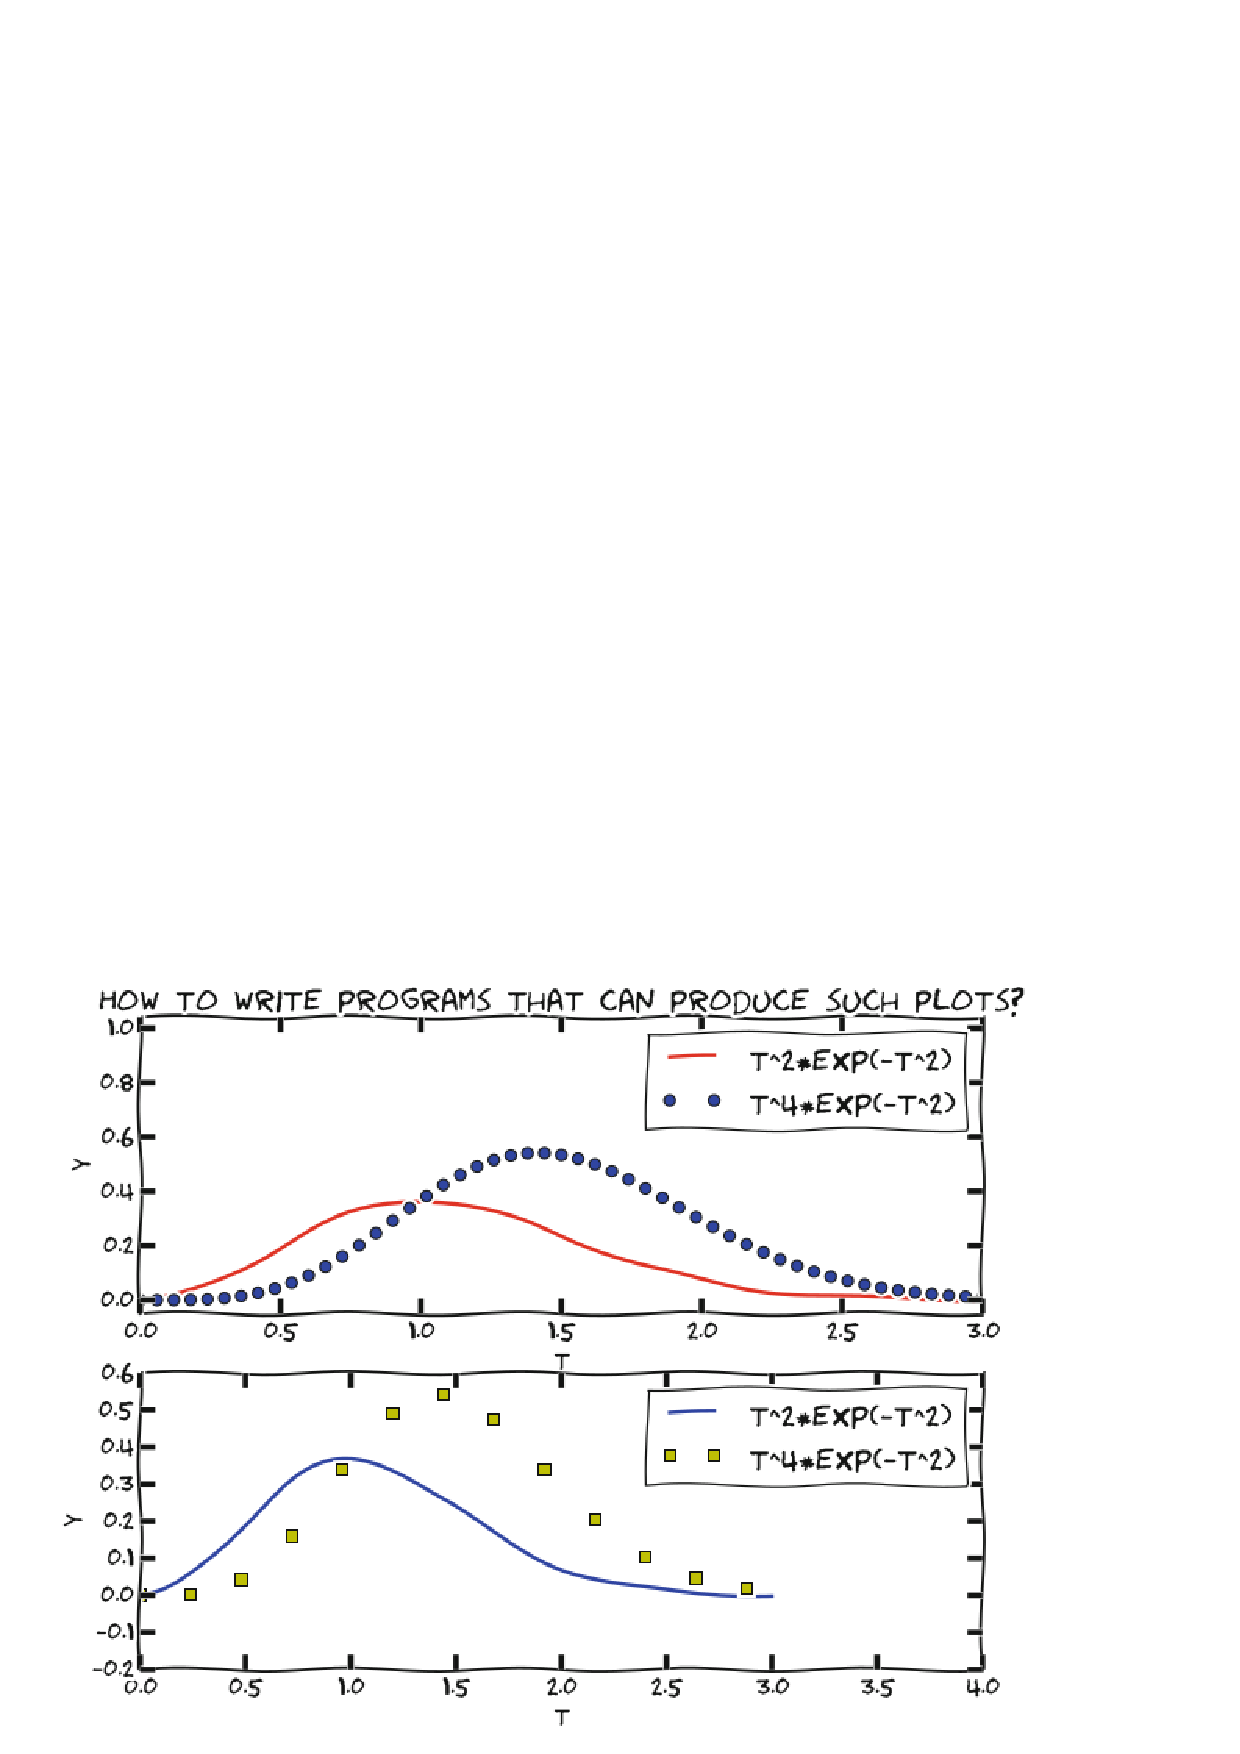
\includegraphics[width=200pt]{chapters/chapter0/figures/manual_graph.png}
    \caption[Desenhando Gráficos Manualmente]{Desenhando Gráficos Manualmente}
\end{figure}

Não somente nas engenharia os profissionais necessitam das habilidades de manipular e exibi-los dados graficamente,
a maioria das pessoas tem experiencias em softwares como Microsoft Excel, Libreoffice Calc, entre outras ferramentas dedicadas.
No entanto, essa interação geralmente é bastante simples, com alguns cliques é possível gerar diversos gráficos para visualização dos dados.

Porém, dada a característica dos dados a serem plotados, faz-se necessário um nível de customização maior, surgindo a necessidade.

Python é uma excelente linguagem para iniciantes, bem como usuários avançados, pois possui uma sintaxe simples e clara. Outro ponto
forte é as bibliotecas de python que apresenta diversas opções para processamento e visualização de dados. Destaca-se inicialmente aqui, duas
bibliotecas que serão utilizadas no inicialmente, a biblioteca para processamento numérico \textbf{numpy}, biblioteca \textbf{scipy} com diversas
funções da área de ciência da computação e \textbf{matplotlib} para visualização dos dados.
\subsection{Instalação do Python}

Para estudar desta matéria, você precisa de uma instalação do Python que atenda ao propósito de aula. A maneira mais rápida de obter uma instalação útil do Python em seu computador Windows ou Mac,
é baixar e instalar o Anaconda (https://www.anaconda.com/). Em muitas distribuições de linux, o Python já é nativo,
caso não seja, aconselha-se a instalação pelo terminal utilizando linha de comando.

\begin{lstlisting}
    $ sudo apt-get install python3
\end{lstlisting}

A versão de Python2 está obsoleta desde janeiro de 2020, sendo assim, nem suporte desde então. Por este motivo aconselha-se
a instalação de Python3.

A instalação de uma biblioteca do Python pode ser dada através do comando:
\begin{lstlisting}
    $ sudo python3 -m pip install numpy
\end{lstlisting}

Há diversas opções de serviços online, como a ferramenta Colab do Google, onde disponibiliza opções com recursos computacionais interessantes,
a uma conta google são oferecidas três opções de hardware, Máquina sem GPU, com GPU e uma Máquina com TPU.

\subsection{Problemas Numéricos com Python}

Para o nosso primeiro exemplo de problema numérico utilizando a linguagem Python, vamos fazer uso da expressão do grafico abaixo.

\begin{equation*}
    y = t^2\exp(-t^2)
\end{equation*}

Neste momento, teremos que recorrer a algumas funções da biblioteca \textbf{numpy}, como \textbf{numpy.exp} e \textbf{numpy.linspace} para gerar um vetor de tempo $t$.

\begin{lstlisting}
    ## importando bibliotecas
    from numpy import exp, linspace
    ## Definindo a funcao
    def yf(t):
        return t**2*exp(-t**2)

    # vetor t, inicio em 0 e fim em 3
    #   com 50 elementos
    t = linspace(0,3,50)

    y = yf(t)
\end{lstlisting}

Assim a variável $y$ recebe $y_f(t)$.

\subsubsection{Plotando Dados}

Dando continuidade ao exemplo anterior, apresentamos aqui outra biblioteca do python, a  \textbf{matplotlib} para visualização dos dados.
Considerando o exemplo acima, temos:

\begin{lstlisting}
    ## importando bibliotecas
    from numpy import exp, linspace
    ## Definindo a funcao
    def yf(t,n):
        return t**n*exp(-t**2)

    # vetor t, inicio em 0 e fim em 3
    #   com 50 elementos
    t = linspace(0,3,50)

    y1 = yf(t,2)
    y2 = yf(t,4)

    # importando o modulo pyplot e renomeando como plt
    import matplotlib.pyplot as plt

    plt.plot(t,y1)
    plt.plot(t,y2, "o")
    plt.xlabel("t")
    plt.ylable("y")
    plt.legend(["T^2*EXP(-T^2)", "T^4*EXP(-T^2)"])
\end{lstlisting}

O resultado esperado será:

\begin{figure}[htb]
    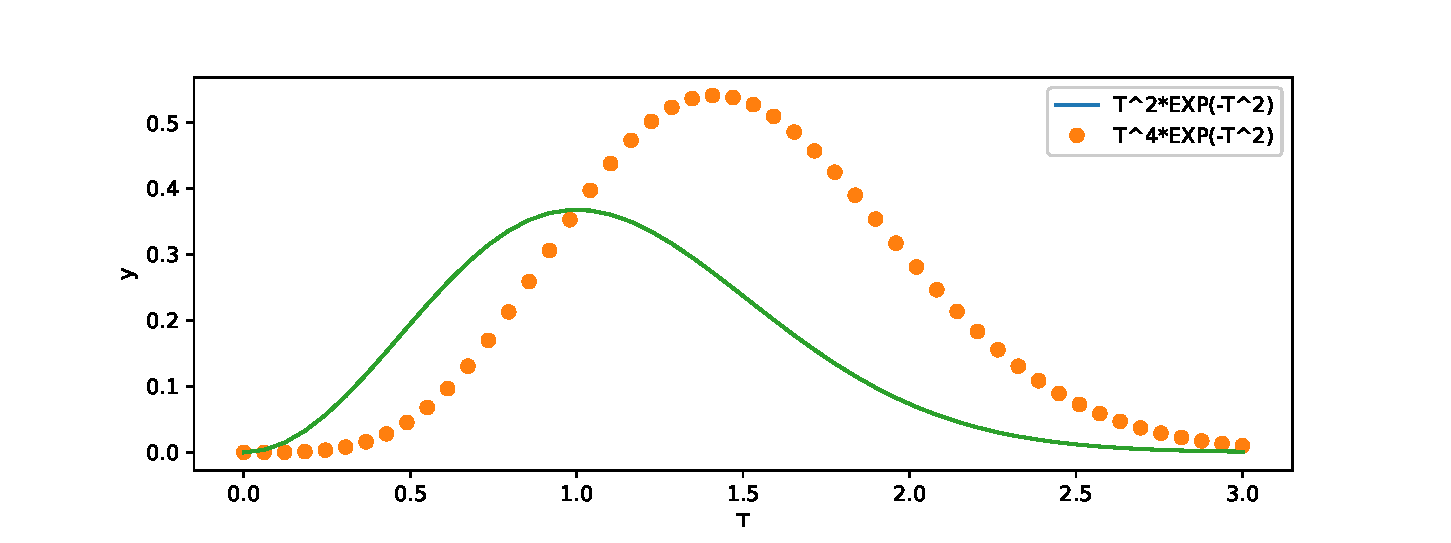
\includegraphics[width=300pt]{chapters/chapter0/figures/python_graph.eps}
    \caption[Desenhando Gráficos Manualmente]{Matplotlib Gráficos}
\end{figure}

A uma série de customizações que podem ser feitas no gráfico, como escrever a legenda em latex, mudança de cores, etc ... Para mais informações consulte a documentação do 
\textbf{matplotlib} na internet.

\subsubsection{Simulação numérica de Sistemas Dinâmicos}

\begin{VF}
    ``Um sistema dinâmico contínuo é um sistema dinâmico cujo estado evolui ao longo do espaço de estado continuamente de acordo com uma regra fixa.''
    
    \VA{Jaime E. Villate}{Introdução aos sistemas dinâmicos, 2007}
    \end{VF}

    Para entender melhor como resolver numericamente um sistemas dinâmicos utilizando uma linguagem de programação, primeiro precisamos recorrer ao problema.

    Aqui será apresentado um problema simples, onde deseja se saber a velocidade de um veículo, considerando limitações impostas pelo seu modelo dinâmico, O veículo está sobre uma superfície plana em condições de rolagem... então é aplicado uma força de tração $u$ ("um empurrão") no sentido do seu movimento, $b$ será o coeficiente de atrito e $m$ a massa.

\begin{figure}[htb]
    \includegraphics[width=300pt]{chapters/chapter0/figures/cruise_control_schematic.png}
    \caption[Desenhando Gráficos Manualmente]{Matplotlib Gráficos}
\end{figure}

Deve-se agora listar as forças com base na física do sistema.

\begin{equation*}
    m\dot{v}+bv=u
\end{equation*}

Substituindo $v$ por $\dot{x}$:

\begin{equation*}
    m\ddot{x}+b\dot{x}=u
\end{equation*}

sendo $x$, posicionamento, $\dot{x}$ velocidade e $\ddot{x}$ aceleração, temos então a função de espaço de estados:

\begin{equation}\label{eq:car}
    \frac{d}{dt}\begin{bmatrix} x_0 \\ x_1 \end{bmatrix} = 
    \begin{bmatrix} 1 & 0\\ -\displaystyle\frac{b}{m} & +\displaystyle\frac{1}{m} \end{bmatrix}
    \begin{bmatrix} x_1 \\ u \end{bmatrix}    
\end{equation}

A solução numérica de Eq. \ref{eq:car} é obtida através de um método de integração, em Python a biblioteca \textbf{scipy} traz os diversos métodos de integração, a função responsável por chamar o integrador é \textbf{odeint}.

\begin{lstlisting}
    import numpy as np
    import matplotlib.pyplot as plt
    from scipy.integrate import odeint

    ## Definindo a funcao carro
    def car(x,t):
        m = 2000
        b = 240
        u = 100
        # inicializando vetor derivadas
        dx = np.zeros(2,)
        dx[0] = x[1]
        dx[1] = 1/m*(-b*x[1]+u)
        return dx

    # vetor t, inicio em 0 e fim em 3
    #   com 100 elementos
    t = np.linspace(0,10,100)
    # condicoes iniciais
    x0 = [0,0]

    # integrador
    x = odeint(car, x0, t)

    # plotando os valores
    plt.plot(t,x[:,0],t,x[:,1])
    plt.xlabel("t")
    plt.legend(["Posicao", "Velocidade"]) 
\end{lstlisting}
 
A solução numérica pode ser vista pelo gráfico abaixo:

\begin{figure}[htb]
    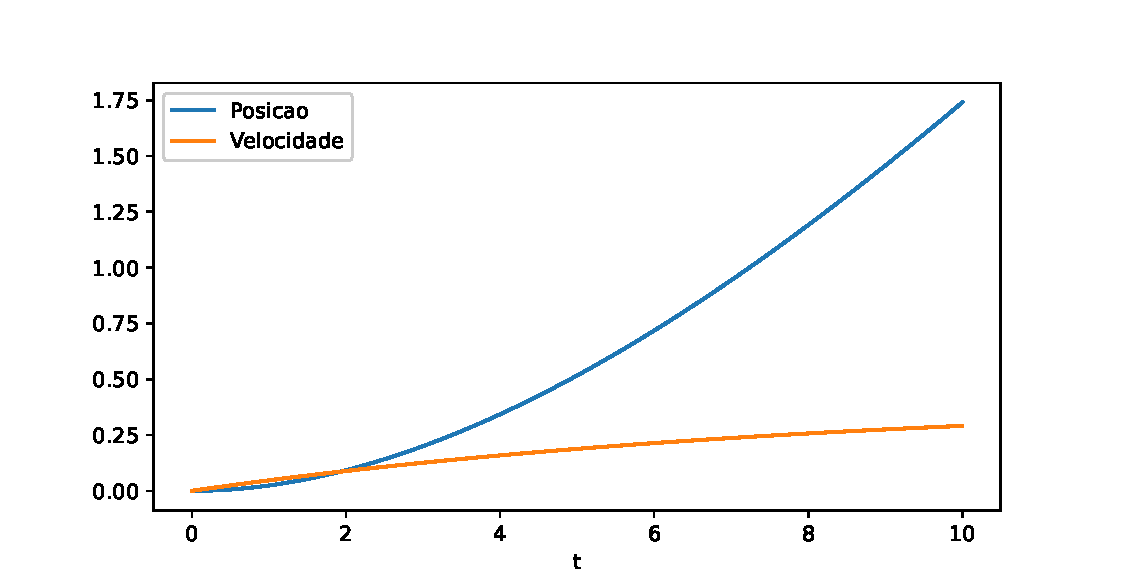
\includegraphics[width=300pt]{chapters/chapter0/figures/exercice_car.eps}
    \caption[Modelo Dinâmico Carro]{Gráfico velocidade e Posicionamento Carro}
\end{figure}

O sistema apresentado possui apenas dois estados, no entanto, sistemas de maior ordem podem ser
simulados utilizando os métodos de integração, como será visto no próximo capítulo.

\begin{shortbox}
    \Boxhead{Exercício de Fixação}
    Com base no sistema do robô demonstrado acima, escreva um programa que simule a situação onde o robô é inicializado em uma rampa com angulo de $\theta=30$ graus, lembre que ele sob da força gravitacional $G=\sin(\theta)mg$, onde $m$ é a massa e $g$ é a
    força gravitacional. Qual vai ser a velocidade e posicionamento final do robô após decorrido 10 segundos. Parâmetros: Força de tração $u=8\text{Nm}$,
    coeficiente de atrito $b=2$ e massa $m=3$.
    \begin{center}
        Resposta:

        \qrcode[height=0.5in]{Posicionamento, Velocidade: -2.0704, -0.2.432}
\end{center}

\end{shortbox}

\subsubsection{Biblioteca Simbólica}

Em algumas situações, faz se interessante utilizar ferramentas para facilitar e/ou simplificar a solução de sistemas de equações. Neste caso utilizaremos a biblioteca \textbf{sympy}, que possui várias ferramentas para solução de equações dinâmicas.

Vamos a um exemplo:

\begin{lstlisting}
    from sympy import *

    # definindo x como uma variavel
    x = symbols('x')
    eq = (sin(x)**2 + cos(x)**)**2

    # expandir equacao eq
    expand(eq)
    # >> sin(x)**4 + 2*sin(x)**2*cos(x)**2 + cos(x)**4

    # simplificar equacao eq
    simplify(eq)
    # >> 1

\end{lstlisting}

Para memorizar o uso da ferramenta de solução de equações simbólicas, vamos a alguns exercícios de fixação.

\begin{shortbox}
    \Boxhead{Exercício de Fixação}
    \begin{enumerate}
        \item  Usando o função \textbf{solve(eq,x)} encontre a solução da função quadrática $ax^2+bx+c=0$.
        \begin{center}
            Solução:

\qrcode[height=1in]{
x = symbols('x')
a = symbols('a')
b = symbols('b')
c = symbols('c')
eq2 = a*x**2+b*x+c
solve(eq2, x)
# >>[(-b + sqrt(-4*a*c + b**2))/(2*a), -(b + sqrt(-4*a*c + b**2))/(2*a)]}
\end{center}

    \item Sendo $x(t)$ uma função no tempo, use o comando \textbf{x = Function('x')} para definir a função $x$ e $t$ como 
    uma variável simbólica. Como o comando \textbf{dsolve(eq, x(t))} ache a solução da equação $\displaystyle\frac{dx(t)}{dt}+x(t)=0$
    \begin{center}
        Solução:

\qrcode[height=1in]{
x = Function('x')
t = symbols('t')
eq = diff(x(t), t) + x(t)
dsolve(eq, x(t))
eq2 = a*x**2+b*x+c
dsolve(eq2, x)
# >>Eq(x(t), C1*exp(-t))}
\end{center}

\end{enumerate}
\end{shortbox}



\section{Glossário}
\begin{Glossary}
\item[360 Degree Review] Performance review that includes feedback from superiors, peers, subordinates, and clients.
% \item[Abnormal Variation] Changes in process performance that cannot be accounted for by typical day-to-day variation. Also referred to as
% non-random variation.
% \item[Acceptable Quality Level (AQL)] The minimum number of parts that must comply with quality standards, usually stated as a percentage.
% \item[Activity] The tasks performed to change inputs into outputs.
% \item[Adaptable] An adaptable process is designed to maintain effectiveness and efficiency as requirements change. The process is
% deemed adaptable when there is agreement among suppliers, owners, and customers that the process will meet
% requirements throughout the strategic period.
\end{Glossary}





\part{Cinemática e Dinâmica de Robôs Móveis}
\chapterauthor{Jeferson J. Lima}{Departamento de Informática (DAINF) \\Universidade Tecnológica Federal do Paraná (UTFPR)}
\chapter{Cinemática e Dinâmica de Robôs Móveis com Rodas}


\section{Introdução}\label{intro}
% 2. Cinemática e Dinâmica de Robôs Móveis com Rodas
% 	2.1 Cinemática Direta e Inversa
% 		2.1.1 Cinemática Direta e Inversa
% 		2.1.1 Cinemática de Robôs Móveis com Rodas
% 	2.2 Restrições de Movimento
% 		2.2.1 Sistemas Holonômicos
% 		2.2.2 Sistemas Não-Holonômicos
% 	2.3 Modelagem de Robô Móvel com restrições de Movimento.
% 3. Controle Moderno para Robótica Móvel
% 	3.1 Lyapunov-based Controle
% 	3.2 SDRE Controle
% 4. Eventos Não Deterministicos em Robótica Móvel
% 	4.1 Estimação de Estados
% 	4.2 Filtro Bayesiano
% 	4.3 Filtro de Kalman
% 		4.3.1 Filtro de Kalman Estendido

A humanidade é facinada pelo movimento das rodas a milhares de anos, isso intriga até os dias de hoje, o homem moderno.
Na matemática há areas expecíficas para descrever o movimento dos corpos, ou para o nosso interesse nesse capítulo, a cinemática dos robôs. 
Um modelo cinemático de um robô, com rodas ou pernas, descreve as relações geometricas entre que dão forma ao próposito deste robô.

Em resumo, os modelos cinemáticos estão relacionadas a como as velodicidades dos elementos do robô interagem entre si e o espaço.


\section{Cinemática Direta e Inversa}\label{intro-ch1}

A Cinemática é a ciência que trata do movimento (geométrico) e das forças que o causam [Craig]. Desta forma, dependendo do ponto de visão,
podemos referênciar a cinemática de um robô atravês de uma referência externa (Cinemática externa), como por exemplo a relação entre o robô e
as coordenadas de um mapa global. Há a possibilidade também, da referência ser o próprio robô, desta forma da-se o nome de
Cinemática Interna, como exemplo, podemos citar a velocidade de rotação em torno do seu eixo ou velocidade das rodas.

Podemos ainda nos aprofundar mais sobre a Cinemática Interna do Robô, onde o espaço de ação das coordenadas definem a forma que se deve tratar o modelo de equações.
Considerando um robô fixo ou móvel com coodenadas generalizadas $\theta_1, \theta_2,..., \theta_n$ localizadas no espaço das \textcolor{red}{juntas ou atuadores (\textit{joint space}) $\mathbf{q}$}. Bem como $x_1, x_2,..., x_n$, o \textcolor{blue}{espaço das tarefas (\textit{task space}) $\mathbf{x}$}, temos então os vetores:

\begin{figure}[!ht]


\begin{tikzpicture}
    \newcommand{\nvar}[2]{%
    \newlength{#1}
    \setlength{#1}{#2}
    }

    % Define a few constants for drawing
    \nvar{\dg}{0.3cm}
    \def\dw{0.25}\def\dh{0.5}
    % Define commands for links, joints and such
    \def\link{\draw [double distance=1.5mm, very thick] (0,0)--}
    \def\joint{%
    \filldraw [fill=white] (0,0) circle (5pt);
    \fill[black] circle (2pt);
    }
    \def\grip{%
    \draw[ultra thick, blue](0cm,\dg)--(0cm,-\dg);
    \fill[blue] (0cm, 0.5\dg)+(0cm,1.5pt) -- +(0.6\dg,0cm) -- +(0pt,-1.5pt);
    \fill[blue] (0cm, -0.5\dg)+(0cm,1.5pt) -- +(0.6\dg,0cm) -- +(0pt,-1.5pt);
    }

    \def\robotbase{%
    \draw[rounded corners=8pt] (-\dw,-\dh)-- (-\dw, 0) --
        (0,\dh)--(\dw,0)--(\dw,-\dh);
    \draw (-0.5,-\dh)-- (0.5,-\dh);
    \fill[pattern=north east lines] (-0.5,-1) rectangle (0.5,-\dh);
    }
    \newcommand{\doublelink}[6]{%
    \robotbase
    \link(#1:#2);
    \joint
    \node[left]{$\color{black}{\theta_1}$};
    \begin{scope}[shift=(#1:#2), rotate=#1]
        \link(#3:#4);
        \joint
        \node[above]{$\color{black}{\theta_2}$};
        \begin{scope}[shift=(#3:#4), rotate=#5]
            \grip
            \node[right]{$\color{blue}{\mathbf{x}_{tool}}$};
        \end{scope}
    \end{scope}
    }

    \doublelink{60}{2}{-90}{2}{-60}{1}
\end{tikzpicture}
    
\caption{Robô - Dois Graus de Liberdade}
\label{fig:2dof-robot}
\end{figure}

Assim sendo, da-se o nome de a \textcolor{red}{Cinemática Direta} quando o robô e descrito como função de entradas como (velocidade das rodas, movimento das juntas, direção das rodas).  Já a \textcolor{blue}{Cinemática Inversa} possibilita projetar um planejamento de movimento, o que significa que as entradas do robô podem ser calculadas para uma sequência de estado do robô desejada.

A relação entre as Cinemática Direta e Cinemática Inversa é obtida através da Matriz Jacobiana do Robô.

\begin{equation*}
    \mathbf{\dot{x}} = \mathbb{J}{\mathbf{\dot{q}}}
    \text{ e, }
    \mathbf{\dot{q}} = \mathbb{J}^{-1}{\mathbf{\dot{x}}}
\end{equation*}

bem como:

\begin{equation*}
    \frac{\text{d}\mathbf{x}}{\text{d}t} = \mathbb{J}\frac{\text{d}\mathbf{q}}{\text{d}t}
    \text{ e, }
    \frac{\text{d}\mathbf{q}}{\text{d}t} = \mathbb{J}^{-1}\frac{\text{d}\mathbf{x}}{\text{d}t}
\end{equation*}

onde $\mathbb{J}$ é dado por:
\begin{equation*}
    \mathbb{J}
    =
    \frac{d \mathbf{f}}{d \mathbf{q}}
    =
    \left[ \frac{\partial \mathbf{f}}{\partial q_1}
        \cdots \frac{\partial \mathbf{f}}{\partial q_n} \right]
    =
    \begin{bmatrix}
        \frac{\partial f_1}{\partial q_1} & \cdots &
        \frac{\partial f_1}{\partial q_n}                   \\
        \vdots                            & \ddots & \vdots \\
        \frac{\partial f_m}{\partial q_1} & \cdots &
        \frac{\partial f_m}{\partial q_n}
    \end{bmatrix}
\end{equation*}

Essa transformação é feita quando necessita-se, por exemplo, controlar um robô utilizando-se das referências de uma ferramenta acoplada a
extremidade do braço robótico. A Cinemática Inversa proporciona que a estratégia de controle seja aplicada na ferramenta até
que o objetivo da tarefa seja alcançado.


\begin{shortbox}
    \Boxhead{Exercício de Fixação}
    Levando em consideração o braço robótico da Figura \ref{fig:2dof-robot}, encontre as equações da cinemática do robô.
    \begin{equation*}
        \begin{split}
            x_f(t) = & l_1\cos(\theta_1)+l_2\cos(\theta_1 + \theta_2) \\            
            y_f(t) = & l_1\sin(\theta_1)+l_2\sin(\theta_1 + \theta_2)
        \end{split}
    \end{equation*}
    
    utilize a biblioteca \textbf{sympy} para solução do jacobiano.
    \begin{center}
        Resposta:

        \qrcode[height=0.5in]{https://ocw.mit.edu/courses/mechanical-engineering/2-12-introduction-to-robotics-fall-2005/lecture-notes/chapter5.pdf}
\end{center}

\end{shortbox} 


\section{Cinemática de Robôs Móveis com Rodas}

\subsection{Cinemática Biciclo}
\subsection{Cinemática Robô Diferencial}
\subsection{Robô Omnidirecional}


\section{Dinâmica com Restrições de Movimento}
\subsection{Sistemas Holonômicos}
\subsection{Sistemas Não-Holonômicos}

\section{Modelagem de Robô Móvel com restrições de Movimento}



\section{Glossary}
\begin{Glossary}
\item[360 Degree Review] Performance review that includes feedback from superiors, peers, subordinates, and clients.
\item[Abnormal Variation] Changes in process performance that cannot be accounted for by typical day-to-day variation. Also referred to as
non-random variation.
\item[Acceptable Quality Level (AQL)] The minimum number of parts that must comply with quality standards, usually stated as a percentage.
\item[Activity] The tasks performed to change inputs into outputs.
\item[Adaptable] An adaptable process is designed to maintain effectiveness and efficiency as requirements change. The process is
deemed adaptable when there is agreement among suppliers, owners, and customers that the process will meet
requirements throughout the strategic period.
\end{Glossary}





% \part{Controle Moderno para Robótica Móvel}
% \chapterauthor{Jeferson J. Lima}{Departamento de Informática (DAINF) \\Universidade Tecnológica Federal do Paraná (UTFPR)}
\chapter{Controle Moderno para Robótica Móvel}


\section{Introdução}\label{intro}

\subsection{Lyapunov-based Controle}
\subsection{SDRE Controle}


% \section{Glossary}
% \begin{Glossary}
% \item[360 Degree Review] Performance review that includes feedback from superiors, peers, subordinates, and clients.
% \item[Abnormal Variation] Changes in process performance that cannot be accounted for by typical day-to-day variation. Also referred to as
% non-random variation.
% \item[Acceptable Quality Level (AQL)] The minimum number of parts that must comply with quality standards, usually stated as a percentage.
% \item[Activity] The tasks performed to change inputs into outputs.
% \item[Adaptable] An adaptable process is designed to maintain effectiveness and efficiency as requirements change. The process is
% deemed adaptable when there is agreement among suppliers, owners, and customers that the process will meet
% requirements throughout the strategic period.
% \end{Glossary}





\part{Eventos Não Determinísticos em Robótica Móvel}
\chapterauthor{Jeferson J. Lima}{Departamento de Informática (DAINF) \\Universidade Tecnológica Federal do Paraná (UTFPR)}
\chapter{Conceitos Básicos}


% \def\iangle{35} % Angle of the inclined plane
\def\down{0}
\def\arcr{0.7cm} % Radius of the arc used to indicate angles
\newcommand\centerofmass{%
    \tikz[radius=0.2em] {%
        \fill (0,0) -- ++(0.2em,0) arc [start angle=0,end angle=90] -- ++(0,-0.4em) arc [start angle=270, end angle=180];%
        \draw (0,0) circle;%
    }%
}

\begin{tikzpicture}[
    force/.style={>=latex,draw=blue,fill=blue},
    axis/.style={densely dashed,gray,font=\small},
    M/.style={rectangle,draw,fill=lightgray,minimum size=0.7cm,thin},
    m/.style={rectangle,draw=black,fill=lightgray,minimum size=0.3cm,thin},
    plane/.style={draw=black,fill=blue!10},
    string/.style={draw=red, thick},
    pulley/.style={thick},
    wheel/.style={fill=black, rounded corners=1.5pt},
]
    %% Free body diagram of M
    \begin{scope}[rotate=\iangle]
        \node[M,transform shape] (M) {\centerofmass};
        % Draw axes and help lines
        {[axis,->]
            \draw (M) -- ++(0,1.3) node(y1_axis)[right] {$y$};
            \draw (M) -- ++(2,0) node[right] {$x$};
            % Indicate angle. The code is a bit awkward.
            \draw[solid,shorten >=0.5pt] (\down-\iangle:\arcr)
                arc(\down-\iangle:\down:\arcr);
            \node at (\down-0.5*\iangle:1.3*\arcr) {$\phi$};
        }
        % Forces
        {[force,->]
            % Assuming that Mg = 1. The normal force will therefore be cos(alpha)
            \draw (M.east) -- ++(1,0) node[above, blue] {$v_M$};
        }
        \draw[wheel] (M.south west) rectangle ++(.4,-.1) node[below]{$v_{M_R}$};
        \draw[wheel] (M.north west) rectangle ++(.4,.1)  node[left]{$v_{M_L}$};
        \draw [-](M) -- ++(0,2) node(CIR)[above] {CIR};
    \end{scope}
    % Draw gravity force. The code is put outside the rotated
    % scope for simplicity. No need to do any angle calculations. 
    \draw[axis,] (M.center) -- ++(1,0) node[below] {};
    %%
    \node[right, gray,font=\small, xshift=8] at (y1_axis) {$\{M\}$};
    %%
    \draw[, ->] (-2,-1) -- ++(4,0) node[below] {$X$};
    \draw[, ->] (-2,-1) -- ++(0,3) node(y_axis)[right] {$Y$};
    \draw[gray, ->] (-2,-1) -- ++(-.5,-.5) node[left] {$Z$};
    \node[left, gray,font=\small, xshift=-10] at (y_axis) {$\{I\}$};
\end{tikzpicture}


 
\section{Introdução}\label{intro::cap3}

A modelagem cinemática e dinâmica fornece uma estimativa dos estados de um sistema real em relação aos valores inciais. No caso da robótica móvel, essa estimativa aplica-se principalmente na determinação da posição de um robô em relação as coordenas iniciais, sendo estas um mapa ou qualquer outro sistema de referência.

A percepção destas coordenadas se dá através de uma série de sensores que fornecem uma estimativa da localização do robô durante determinado movimento. Esta predição dos estados é executada interativamente em intervalos de tempo, determinados pela frequência de operação dos sensores. 

Assim, a crença do estado atual do robô é determinada em função dos dados dos sensores, bem como, do modelo de sistema atribuído ao robô. A integração entre os dados observáveis e integração de estados do modelo é feita através da proposta de alguns filtros que serão discutidos na sequência. 

subsection{Filtro de Bayes}

O Filtro de Bayes é um dos algoritmos mais utilizados em diversas técnicas de auto-localização onde pretende-se resolver a manutenção da crença da posição de um robô. O algoritmo calcula a densidade de probabilidade que se traduz na crença do robô a partir de dados dos sensores e o modelo de controle do robô  \cite{thrun2006probalistic}. A solução deste problema de auto-localização, utilizando-se da inferência bayesiana com objetivo de encontrar o valor esperado da posição em cada instante de tempo, conforme a \eq{eq:bayes1}.

\begin{equation}
    \label{eq:bayes1}
    \hat X_t = E\left[X_t| z_t, u_t\right] = \displaystyle \int\limits_x x P(X_t = x| z_t, u_t)\text{d}x
\end{equation}

Para este problema, o algoritmo do Filtro de Bayes apresenta-se como uma forma recursiva, conforme a \eq{eq:bayes2}, onde $\text{Bel}(x_t)$ representa a função densidade da crença no tempo $t$ e $\text{Bel}(x_{t-1})$ a função no intervalo de tempo anterior. A relação entre o intervalo de tempo das interações do filtro será definida, conforme citado acima, pela velocidade de operação dos sensores envolvidos, aqui apresentados como $z_t$. O termo $u_t$ representa a variável de ação do modelo ou variável de controle.

\begin{equation}
    \label{eq:bayes2}
    \text{\text{Bel}}(x_t) = \eta P(z_t| x_t) \int P(x_t| u_t, x_{t-1}) \text{Bel}(x_{t-1})\text{d}x_{t-1}
\end{equation}

A esta primeira fase do algoritmo, a qual calcula a distribuição em relação à crença dos estados $x_{t-1}$ e $u_t$, é chamada de predição e o resultado da função crença é dada por $\overline{\text{Bel}}(x_t)$.

Na segunda fase, chamada aqui de correção, a crença $\overline{\text{Bel}}(x_t)$ é multiplicada pela probabilidade dos estados observados em relação aos sensores $z_t$.

\begin{algorithm}[H]
    \caption{Filtro de Bayes}
    \begin{algorithmic}[1]
    \Procedure{predição}{$\text{Bel}, u_t$}
        \State $\overline{\text{Bel}}= \displaystyle\int P(x_t| u_t, x_{t-1})\text{Bel}(x_{t-1})\text{d}x_t$
    \EndProcedure
    \Procedure{Correção}{$\overline{\text{Bel}}, z_t$}
        \State ${\text{Bel}}= \displaystyle\textcolor{white}{\int}  \eta P(z_t| x_{t})\overline{\text{Bel}}(x_{t})$
    \EndProcedure
    \State Normatiza $\eta \displaystyle\int \text{Bel}(x_t)\text{d}x_t = 1$
    \State \textbf{Retorne} $\text{Bel}(x_t)$
    \end{algorithmic}
    \label{algo:bayes}
\end{algorithm}

O \algo{algo:bayes} finaliza com a crença normatizada e a estimativa da posição do robô é calculada. O algoritmo do Filtro de Bayes apresentado aqui é aplicável apenas a uma classe de problemas simples, no entanto, serve de base para implementações mais complexas onde a cinemática e dinâmica dos sistemas são consideradas, como no exemplo do Filtro de Kalman a ser apresentado abaixo.

\subsection{Filtro de Kalman}

O Filtro de Kalman é provavelmente a implementação mais aplicada com base no Filtro de Bayes. Proposto por Rudolph Emil Kalman, em 1950 como técnica para filtragem e predição de sistemas lineares. O Filtro proposto por Kalman resolve o problema de observação dos sensores externos do robô, considerando inerentes a leitura dos sensores. \cite{thrun2006probalistic,romero2014robotica}.

A garantia da densidade de probabilidade, apresentada em \eq{eq:bayes2}, é dada por uma aproximação do método apresentado anteriormente. Nesta aproximação o modelo de movimento do robô e o modelo do observador, com base nos sensores, é representado por densidades gaussianas multivariáveis.

A função de densidade gaussiana $P(X = x)$, sendo $X$ um vetor, pode ser expressa na seguinte forma ${P(X = x) \sim N(\mu, \sigma^2)}$, onde $\mu$ representa a média e $\sigma^2$ a variância da distribuição, conforme a  \eq{eq:gauss1}.

\begin{equation}
    \label{eq:gauss1}
    P(X = x) = \dfrac{1}{\sqrt{2\pi\sigma^2}}\cdot 
    \exp\left\{-\frac{(x-\mu)^2}{2\sigma^2}\right\}
\end{equation}

A \fig{fig::gauss1} apresenta três funções de densidade gaussiana, com os valores respectivamente para $\mu_i = \{0,0,-2\}$ e $\sigma^2_i = \{1,2,1\}$.

\begin{figure}[!ht]
    \centering
    \input{chapters/chapter3/figures/gauss_1d_image.tex}
    \caption{Representação de três funções de Distribuição Normal}
    \label{fig::gauss1}
\end{figure}

Um dos requisitos para aplicação do Filtro de Kalman é que o modelo determinístico de observação seja linear para uma correta aproximação com a densidade de probabilidade, conforme é mostrado na  \eq{eq::linear1d}.

\begin{equation}
    \label{eq::linear1d}
    \left.
    \begin{aligned}
            X & \sim N\left(\mu, \sigma^2\right)\\
            Y & = aX + b\\
    \end{aligned} \right\}
    \quad \Rightarrow \quad Y \sim N\left(a\mu+b\right)
\end{equation}

Os coeficientes $a$ e $b$ são coeficientes lineares do modelo. A \eq{eq::linear1d} possui apenas um estado, no entanto, sistemas complexos são tipicamente representados diversos estados e diversos sensores.
Sistemas robóticos possuem vários estados, sendo assim a densidade de probabilidade ${P(\mathbf{x}) \sim N(\boldsymbol{\mu}, \textstyle\sum)}$ é formada por uma  multivariável, onde $\boldsymbol{\mu}$ representa o vetor das médias e ${\textstyle\sum}$ a matriz de covariância, conforme pode ser visto na  \eq{eq::linearNd}.

\begin{equation}
    \label{eq::linearNd}
    P(\mathbf{x}) =\frac{1}{\sqrt{(2\pi)^{d}|\sum|}}\exp\left\{-\frac{1}{2} (\mathbf{x}-\boldsymbol\mu)^T\textstyle\sum{}^{-1}(\mathbf{x}-\boldsymbol\mu)\right\}
\end{equation}

Desta forma, a \fig{fig::gauss2} apresenta a distribuição normal para um sistema bivariável.

\begin{figure}[!ht]
    \centering
    \input{chapters/chapter3/figures/gauss_2d_image.tex}
    \caption{Distribuição Normal Bivariável}
    \label{fig::gauss2}
\end{figure}

A equação da função densidade de probabilidade e mostrada pela \eq{eq:multi}.

\begin{equation}
    \left.
    \begin{aligned}
            X & \sim N\left(\boldsymbol\mu, \textstyle\sum\right)\\
            Y & = {A}_tX + {B_t}\\
    \end{aligned} \right\}
    \quad \Rightarrow \quad Y \sim N\left( {A_t}\boldsymbol\mu+B_t, {A_t}\textstyle\sum {A_t}^T \right)
    \label{eq:multi}
\end{equation}

Para o caso multivariável, ${A_t}$ e ${B_t}$ são matrizes $n \times n$ e $n \times l$, respectivamente, sendo $n$ o número de estados e $l$ o número de variáveis de controle.

Definida a funções de densidade de probabilidade para um sistema multivariável, tem-se agora que definir o modelo do sistema. No modelo estocástico do sistema do robô, as incertezas serão acrescentadas, conforme visto pela  \eq{eq::mdinamic}.

    \begin{equation} 
        \label{eq::mdinamic}
        \begin{aligned}
            x_t &= {A}_t x_{t-1} + {B}_t u_t +  w_t\\ 
        z_t &= {C}_t x_t + v_t
        \end{aligned}
    \end{equation}

\noindent sendo:

\begin{center}
    \begin{tabular}{ r | l }
        ${A}_t$ & Matriz $(n \times n)$ que descreve os estados do modelo.      \\
        ${B}_t$ & Matriz $(n \times l)$ que descreve os estados do controle.    \\
        ${C}_t$ & Matriz $(k\times n)$ sendo os estados de $x_t$.               \\
        $w_t$   & Variável aleatória com distribuição normal e covariância ${Q}$. \\
        $v_t$   & Ruído aleatório com distribuição normal, covariância de ${R}$.
    \end{tabular}
\end{center}

Definidas as variáveis do sistema, necessita-se agora desenvolver a metologia para proposta de filtro a ser aplicado. A evolução da proposta, com base na \eq{eq:bayes2}, segue os seguintes passos.

\begin{equation*}
    \begin{array}{ll}
        \text{Teorema} & \Rightarrow\textcolor{white}{\displaystyle\int}\text{Equações} \\
        Bel(x_t) & \Rightarrow\textcolor{white}{\displaystyle\int} P(x_t| u_1, z_1,  \cdots, z_t) \\
        Bayes & \Rightarrow\textcolor{white}{\displaystyle\int} \eta P(z_t|x_t,  u_1, z_1,  \cdots,  u_t)P(x_t, u_1, z_1, \cdots, u_t) \\
        Markov & \Rightarrow\textcolor{white}{\displaystyle\int} \eta P(z_t|x_t)P(x_t, u_1, z_1, \cdots, u_t) \\
        P. Total & \Rightarrow\textcolor{white}{\displaystyle\int} \eta P(z_t|x_t)\displaystyle\int P(x_t| u_1, z_1, \cdots, u_t,x_{t-1})P(x_{t-1}| u_1, z_1, \cdots, u_t)\text{d}x_{t-1}\\
        Markov & \Rightarrow\textcolor{white}{\displaystyle\int} \eta P(z_t|x_t) \displaystyle\int P(x_t| u_t,x_{t-1})P(x_{t-1}| u_1, z_1, \cdots, u_t)\text{d}x_{t-1} \\
        Markov & \Rightarrow\textcolor{white}{\displaystyle\int} \eta P(z_t|x_t) \displaystyle\int P(x_t| u_t,x_{t-1}){P(x_{t-1}| u_1, z_1, \cdots, z_{t-1}}){\text{d}x_{t-1}} \\
    \end{array}   
\end{equation*}

Temos então a equação resultante na \eq{eq:kalmbayes}.

\begin{equation}
    \textcolor{blue}{\text{Bel}(x_t)} =\eta \textcolor{purple}{P(z_t|x_t)}\displaystyle\int \textcolor{red}{P(x_t| u_t,x_{t-1})}\textcolor{gray}{\text{Bel}(x_{t-1})}\text{d}x_{t-1}
    \label{eq:kalmbayes}
\end{equation}

A \fig{fig::kalm1} demonstra graficamente a \eq{eq:kalmbayes}, com relação função de densidade de probabilidade em relação aos estados do robô.
    
\begin{figure}[!ht]
    \centering
        \begin{tikzpicture}[
      declare function={
        normalpdf(\x,\mu,\sigma)=
        (2*3.1415*\sigma^2)^(-0.5)*exp(-(\x-\mu)^2/(2*\sigma^2));
      },
      hplot/.style={ycomb, mark=o, dashed}, ,scale=0.8]
    
      \begin{axis}[
        width=10cm, height=5.5cm,
        samples=50,
        legend style={draw=none, fill=none},
        domain=-6:9,
        legend cell align=left,
        xmin=-7, xmax=11]
    
        \addplot [smooth, thick, red] {normalpdf(x,-2,2)} node[] {};
        \addplot [smooth, black]      {normalpdf(x,0,2)} node[] {};
        \addplot [smooth, blue]       {normalpdf(x,-1,1.3)} node[] {};
        \legend{$P( x_t | u_t,x_{t-1})$ \\ $P(z_t | x_t)$ \\ $\text{Bel}(x_t)$\\};
      \end{axis}
    \end{tikzpicture}
    \caption{Exemplo Gráfico da Solução da \eq{eq:kalmbayes}}
    \label{fig::kalm1}
\end{figure}

O estado inicial do sistema é fator crucial para convergência do algoritmo de Kalman, sendo definido por:

\begin{equation}
    \text{Bel}(x_0) = N\left(x_0, \mu_o, {\textstyle\sum} _0\right)
\end{equation}

A proposta de filtro é aplicável, apenas se o sistema é observável, desta forma a verificação de tal condição é dada pelo posto  da matriz $\mathcal {O}$ é igual a $n$, conforme mostrado abaixo.
\begin{equation*}
    \mathcal {O}={\begin{bmatrix}C_t\\C_tA_t\\C_tA^{2}_t\\\vdots \\C_tA^{n-1}_t\end{bmatrix}, \quad \text{se }(\text{posto}(\mathcal {O}})) = n
\end{equation*}

Dado que o sistema é observável, temos a função de probabilidade expressa pela \eq{eq:bayes01}:

\begin{equation}
    \label{eq:bayes01}
        p(x_t| u_t, x_{t-1})= N\left(x_t; Ax_{t-1}+ Bu_t, Q\right)
\end{equation}   

Expandindo a equação, na sua forma completa, obtemos a \eq{eq:bayes02}:

\begin{equation}   
    \label{eq:bayes02}
    \begin{matrix}
        \overline{\text{Bel}}(x_t)  & = \displaystyle\int P(x_t|u_t, x_{t-1}) & \text{Bel}(x_{t-1})\text{d}x_{t-1} \\
        & \quad\quad\quad\quad\quad \Downarrow & \quad\quad\quad\Downarrow \\
        & \sim N\left(x_t; A_t x_{t-1}+ B_tu_t, Q_t\right) & \sim N\left(x_{t-1}; \mu_{t-1}, \textstyle\sum {}_{t-1}\right) \\
    \end{matrix}
\end{equation}

O termo $\text{Bel}(x_{t-1})$ representa a função de crença do sistema a \textit{priori} e $\overline{\text{Bel}}(x_t)$ a \textit{posteriori}. Aqui podemos recorrendo à função de densidade de probabilidade para sistemas multivariáveis, temos então a expressão:

\begin{equation}
    \label{eq:bayes03}
    P(\mathbf{x}) = \frac{1}{\sqrt{(2\pi)^{d}|\sum|}}\exp\left\{-\frac{1}{2} (\mathbf{x}-\mu)^T\textstyle\sum{}^{-1}(\mathbf{x}-\mu)\right\}
\end{equation}        

Aplicando a \eq{eq:bayes03} na \eq{eq:bayes02}, obtemos a \eq{eq:bayes04}.

\begin{equation}
    \begin{matrix}
        \label{eq:bayes04}
        \overline{\text{Bel}}(x_t)= &  \eta \displaystyle\int \exp\left\{  -\frac{1}{2} \left(x_t - A_t x_{t-1} - B_t u_t\right)^T Q_t \left(x_t - A_t x_{t-1} - B_t u_t\right)  \right\} \\
        & \quad\exp\left\{ -\displaystyle\frac{1}{2} \left(x_{t-1} - \mu_{t-1}\right)^T \textstyle\sum {}_{t-1} \left(x_{t-1} - \mu_{t-1}\right)  \right\}\text{d}x_{t-1}
    \end{matrix}
\end{equation}

Agora, a \eq{eq:bayes04} pode ser representada por:

\begin{equation}
    \overline{\text{Bel}}(x_t)= \eta \displaystyle\int \exp\left\{ -L_t \right\}\text{d}x_{t-1}
\end{equation}

O funcional $L_t$ é expresso por:

\begin{equation}
    \begin{matrix}
        L_t&  = & \displaystyle\frac{1}{2} \left(x_t - A_t x_{t-1} - B_t u_t\right)^T Q_t \left(x_t - A_t x_{t-1} - B_t u_t\right) \\
        & & \quad\quad + \displaystyle\frac{1}{2} \left(x_{t-1} - \mu_{t-1}\right)^T \textstyle\sum {}_{t-1} \left(x_{t-1} - \mu_{t-1}\right)
    \end{matrix}
\end{equation}

Percebe-se que o funcional $L_t$ é uma função quadrática, representada pelos termos dentro da integral. A solução do funcional $L_t$ nos fornece dois termos importantes para o algoritmo do filtro de Kalman, o valor médio $\left(\mu_t\right)$ e a matriz de covariância $\left(\sum_t\right)$, conforme a \eq{eq:bayes05}.

\begin{equation}
    \overline{\text{Bel}} = 
    \left\{
    \begin{aligned}
            \overline{\mu}_t & = A_t\mu_{t-1} + B_t u_t\\
            \overline{\textstyle\sum}_t & = A_t {\textstyle\sum}_{t-1} A_t^T+ Q_t\\
    \end{aligned} \right.
    \label{eq:bayes05}
\end{equation}

Através da \eq{eq:bayes05}, definimos o primeiro passo do Filtro de Kalman, chamado aqui de correção. A parte de correção fez a estimativa dos estados do sistema em função do seu modelo.
A segunda parte a ser definida é da fase de correção, onde o valores dos sensores $z_t$ terão a função de reduzir o erro de estimação definido no primeiro passo.

Assim, relembrando as equações do sistema, definidas pela \eq{eq::mdinamic}, temos então a \eq{eq:bayes10} de saída do sistema.

\begin{equation}
    z_t = C_t x_t + v_t
    \label{eq:bayes10}    
\end{equation}

Apresentada a equação linear da saída do observador de estados, temos a função de probabilidade na \eq{eq:bayes11}.

\begin{equation}
    P(z_t| x_t)= N\left(z_t; C_t x_t, R_t\right)
    \label{eq:bayes11}
\end{equation}   

Utilizando-se do filtro de Bayes, temos a \eq{eq:bayes12}.

\begin{equation}
    \label{eq:bayes12}
    \begin{matrix}
        \text{Bel}(x_t) = &  \eta & P(z_t| x_t) & \overline{\text{Bel}}(x_t) \\
        & & \quad \Downarrow & \quad\Downarrow \\
        & & \sim N\left(z_t; C_t x_t, R_t\right) & \sim N\left(x_t; \overline{\mu}_t, \overline{\textstyle\sum}_t\right) \\
    \end{matrix}
\end{equation}

Da mesma forma, pode-se então aplicar a \eq{eq:bayes12} na \eq{eq:bayes02}, onde obtemos a \eq{eq:bayes13}.

\begin{equation}
    \label{eq:bayes13}
    \begin{matrix}
        \text{Bel}(x_t)  & = \eta & \exp\left\{  -\displaystyle\frac{1}{2} \left(z_t - C_t x_t\right)^T R_t \left(z_t - C_t x_t\right)  \right\} \\
        & & \exp\left\{ -\displaystyle\frac{1}{2} \left(x_t - \overline{\mu}_t\right)^T \overline{\textstyle\sum}_t^{-1} \left(x_t - \overline{\mu}_t\right) \right\}
    \end{matrix}
\end{equation}

Podemos então, substituir a \eq{eq:bayes13} com o funcional $J_t$, conforme mostrado na \eq{eq:bayes15}.

\begin{equation}
    \text{Bel}(x_t)  = \eta  \exp\left\{-J_t\right\}
    \label{eq:bayes15}
\end{equation}

\noindent sendo $J$ expresso por:

\begin{equation}
    J_t = \displaystyle\frac{1}{2} \left(z_t - C_t x_t\right)^T R_t \left(z_t - C_t x_t\right)  +
    \displaystyle\frac{1}{2} \left(x_t - \overline{\mu}_t\right)^T \overline{\textstyle\sum}_t^{-1} \left(x_t - \overline{\mu}_t\right)
\end{equation}

A solução do funcional $J_t$ é expressa pela \eq{eq:bayes14}.

\begin{equation}
    \overline{\text{Bel}} = 
    \left\{
    \begin{aligned}
            \mu_t & = \overline{\mu}_t + K_t(z_t -C_t \overline{\mu}_t)\\
            \textstyle\sum_t & = (I-K_tC_t)\overline{\textstyle\sum}_t \\
    \end{aligned} \right.
    \label{eq:bayes14}
\end{equation}

A matriz $K_t$, representa o ganho do observador, a letra $K$ é utilizada aqui em homenagem a Rudolph Kalman. Desta forma, o ganho ótimo é obtido pela \eq{eq:bayes16}.

\begin{equation}
    \label{eq:bayes16}
    K_t = \overline{\textstyle\sum}_tC_t^T(C_t\overline{\textstyle\sum}_tC_t^T+R_t)^{-1}
\end{equation}

A implementação do algoritmo do Filtro de Kalman pode ser vista no \algo{algo:kf}.

\begin{algorithm}[H]
    \caption{Kalman-Filter}
    \begin{algorithmic}[1]
    \Procedure{Predição}{$\mu_{t-1}, {\textstyle\sum}_{t-1}, u_t$}
        \State $\overline{\mu}_t = A_t\mu_{t-1} + B_t u_t$
        \State $ \overline{\textstyle\sum}_t = A_t {\textstyle\sum}_{t-1} A_t^T+ Q_t$ 
        \State \textbf{Retorne} $\left(\overline{\mu}_t, \overline{\textstyle\sum}_t\right)$
    \EndProcedure
    \Procedure{Correção}{$\overline{\mu}_{t}, \overline{\textstyle\sum}_{t}, z_t$}
        \State $K_t = \overline{\textstyle\sum}_tC_t^T(C_t\overline{\textstyle\sum}_tC_t^T+R_t)^{-1}$
        \State $\mu_t  = \overline{\mu}_t + K_t(z_t -C_t\overline\mu_t)$
        \State{$\textstyle\sum_t = (I-K_tC_t)\overline{\textstyle\sum}_t$}
        \State \textbf{Retorne} $\left(\mu_t, \textstyle\sum_t\right)$
    \EndProcedure
    \end{algorithmic}
    \label{algo:kf}
\end{algorithm}

Embora a implementação do \algo{algo:kf} seja relativamente simples, no que dizer respeito a implementação computacional, a maioria dos sistemas reais não são lineares. Desta forma, a proposta para solução do filtro em sistemas dinâmicos não lineares se apresenta como EKF (do inglês, \textit{Extended Kalman Filter}).


\subsection{Extended Kalman Filter}

A proposta do EKF se aplica também quando as equações que representam a dinâmica do sensor são representadas por equações não lineares.

Neste caso, o filtro de Kalman pode não mais produzir uma estimativa de estado ideal. Para contornar o problema das não linearidades, propões se o método de linearização do sistema, conforme a \eq{eq:ekf1}.

\begin{equation}
    \begin{split}
    x_t = & g(u_t, x_{t-1})\\
    z_t = & h(x_t)
    \end{split}
    \label{eq:ekf1}
\end{equation}
    
\noindent onde $g(u_t, x_{t-1})$ e $h(x_t)$ são funções não lineares que representam, consecutivamente, 
o modelo do sistema e o modelo dos sensores.

O método de linearização se da ao encontrar a função linear do sistema no ponto $\textcolor{red}{a}$ através da Expansão da Série de Taylor, conforme demonstrado na \eq{eq:taylor1}.

\begin{equation}
    f(x,a) = \textcolor{red}{f(a) + \left. \frac{\partial f(x)}{\partial x} \right\vert_{x=a}(x-a)}
    \textcolor{gray}{+\frac{1}{2!}\left. \frac{\partial^2 f(x)}{\partial^2 x} \right\vert_{x=a}(x-a)^2 + \cdots}
    \label{eq:taylor1}
\end{equation}

A \fig{fig:taylor} demonstra graficamente a linearização pelo primeiro termo da Série de Taylor.

\begin{figure}[!ht]
    \centering
    \includegraphics[width=0.8\textwidth]{chapters/chapter3/figures/taylor.pdf}
    \caption{Série de Taylor - Linearização}
    \label{fig:taylor}
\end{figure}

Para o EKF, apenas a aproximação de primeira ordem é utilizada, conforme \eq{eq:taylor1} e \eq{eq:taylor2}.

\begin{equation}
    \label{eq:taylor2}
    \begin{split}
        g(u_t, x_{t-1}) \approx & g(u_t, \mu_{t-1}) + \frac{\partial g(u_t, \mu_{t-1}) }{\partial x_{t-1}}(x_{t-1}-\mu_{t-1}) \\
        g(u_t, x_{t-1}) \approx & g(u_t, \mu_{t-1}) + \color{red}{G_t}(x_{t-1}-\mu_{t-1})
    \end{split}
\end{equation}

\noindent onde $\color{red}G_t$ é calculado pela Matriz Jacobiana.

O mesmo método é utilizado para equação que representa a saída do sistema, temos \eq{eq:taylor4}.

\begin{equation}
    \label{eq:taylor4}
    \begin{split}
        h(x_t) \approx & h(\overline{\mu}_t) + \frac{\partial h(\overline{\mu}_t) }{\partial x_{t}}(x_{t}-\overline{\mu}_{t}) \\
        h(x_t) \approx & h(\overline{\mu}_t) + \color{blue}{H_t}(x_{t}-\overline{\mu}_{t})
    \end{split}
\end{equation}

\noindent onde $\color{blue}H_t$ é calculado pela Matriz Jacobiana.

A matriz Jacobiana demonstrada em $G_t$ e $H_t$ é expressa na forma generalizada pela \eq{eq:taylor5}.

\begin{equation}
    \label{eq:taylor5}
    \mathbb{J}
    =
    \frac{d \mathbf{f}}{d \mathbf{x}}
    =
    \left[ \frac{\partial \mathbf{f}}{\partial q_1}
        \cdots \frac{\partial \mathbf{f}}{\partial x_n} \right]
    =
    \begin{bmatrix}
        \frac{\partial f_1}{\partial x_1} & \cdots &
        \frac{\partial f_1}{\partial x_n}                   \\
        \vdots                            & \ddots & \vdots \\
        \frac{\partial f_m}{\partial x_1} & \cdots &
        \frac{\partial f_m}{\partial x_n}
    \end{bmatrix}
\end{equation}

Desta forma, pode-se reescrever o \algo{algo:kf} através da linearização do sistema pelo Algoritmo \ref{algo:ekf}.

\begin{algorithm}[H]
    \caption{Extended-Kalman-Filter}
    \begin{algorithmic}[1]
    \Procedure{Predição}{$\mu_{t-1}, {\textstyle\sum}_{t-1}, u_t$}
        \State $\overline{\mu}_t = g(u_t, \mu_{t-1})$
        \State $ \overline{\textstyle\sum}_t = G_t {\textstyle\sum}_{t-1} G_t^T+ Q_t$ 
        \State \textbf{Returne} $\left(\overline{\mu}_t, \overline{\textstyle\sum}_t\right)$
    \EndProcedure
    \Procedure{Correção}{$\overline{\mu}_{t}, \overline{\textstyle\sum}_{t}, z_t$}
        \State $K_t = \overline{\textstyle\sum}_tH_t^T(H_t\overline{\textstyle\sum}_tH_t^T+R_t)^{-1}$
        \State $\mu_t  = \overline{\mu}_t + K_t(z_t -h(\overline\mu_t))$
        \State{$\textstyle\sum_t = (I-K_t H_t)\overline{\textstyle\sum}_t$}
        \State \textbf{Returne} $\left(\mu_t, \textstyle\sum_t\right)$
    \EndProcedure
    \end{algorithmic}
    \label{algo:ekf}
\end{algorithm}

A implementação do \algo{algo:ekf} possibilita a implementação do Filtro de Kalman em sistemas não lineares, como os exemplos de robótica móvel apresentados nessa sessão. Além da modelagem do robô, linearização do modelo, faz-se necessário também a modelagem e linearização dos sensores utilizados no sistema. A implementação dos EKF minimizam as incertezas paramétricas da proposta de robô com um sistema de equações não lineares.
% % \part{Ambiente de Simulação}

% \part{Localização e Mapeamento Simultâneos}

% \part{Robôs Bípedes}

% \part{Robôs Aéreos}

\bibliographystyle{plain}
\bibliography{\BIBREF} 

% \printindex

\end{document}


% 1. Introdução a Robótica Móvel
% 	1.1 Primeiros Passos com a Linguagem Python
% 		1.1.1 Plotando Dados
% 		1.1.2 Simulação de Sistemas Dinâmicos
% 		1.1.3 Biblioteca simbólica
% 2. Cinemática e Dinâmica de Robôs Móveis com Rodas
% 	2.1 Rotação, Translação e Transformação Homogênea
% 		2.2.1 Orientação e Rotação
% 		2.2.2 Translação e Rotação
% 		2.2.3 Transformação Homogênea
% 	2.2 Cinemática Direta e Inversa
% 		3.2.1 Cinemática Direta e Inversa
% 		3.2.2 Cinemática de Robôs Móveis com Rodas
% 	2.3 Restrições de Movimento
% 		2.3.1 Sistemas Holonômicos
% 		2.3.2 Sistemas Não-Holonômicos
% 	    2.3.3 Modelagem de Robô Móvel com restrições de Movimento.
% 3. Controle Moderno para Robótica Móvel
% 	3.1 Lyapunov-based Controle
% 	3.2 SDRE Controle
% 4. Eventos Não Deterministicos em Robótica Móvel
% 	4.1 Estimação de Estados
% 	4.2 Filtro Bayesiano
% 	4.3 Filtro de Kalman
% 		4.3.1 Filtro de Kalman Estendido


% Proposta Inicial
% Introdução a Robótica Móvel
%  1.1 Primeiros Passos com a Linguagem Python
%  1.1.1 Plotando Dados
%  1.1.2 Simulação de Sistemas Dinâmicos
%  1.1.3 Biblioteca simbólica
%  1.2 Rotação, Translação e Transformação Homogênea
%  1.2.1 Orientação e Rotação
%  1.2.2 Translação e Rotação
% 2. Cinemática e Dinâmica de Robôs Móveis com Rodas
%  2.1 Cinemática Direta e Inversa
%  2.1.1 Cinemática Direta e Inversa
%  2.1.1 Cinemática de Robôs Móveis com Rodas
%  2.2 Restrições de Movimento
%  2.2.1 Sistemas Holonômicos
%  2.2.2 Sistemas Não-Holonômicos
%  2.3 Modelo De um Robô Móvel com restrições de Movimento.
% 3. Controle Moderno para Robótica Móvel
%  3.1 Lyapunov-based Controle
%  3.2 SDRE Controle
% 4. Eventos Não Determinísticos em Robótica Móvel
%  4.1 Estimação de Estados
%  4.2 Filtro Bayesiano
%  4.3 Filtro de Kalman
%  4.3.1 Filtro de Kalman Estendido